\section{$\exists$-step}



\begin{frame}{Parallel Plans are (Still) Bad!}
(Re-)Consider the following (single) planning problem:
\begin{center}\begin{tikzpicture}[scale=1.0]
    \tikzstyle{N}=[draw,circle,minimum size=4pt,inner sep=0pt]
  
  \node[N,blue] (A1) at (0,0) {C};
  \node[N] (A2) at (2,0) {B}; \node at (2.5,0) {\faArchive};
  \node[N] (A3) at (1,2) {A}; \node at (0.5,2) {\faTruck};
  \draw (A1) -- (A2);
  \draw (A2) -- (A3);
  \draw (A3) -- (A1);

  \node[N] (B1) at (5,0) {F}; \node at (4.5,0) {\faTruck};
  \node[N,blue] (B2) at (7,0) {E};
  \node[N] (B3) at (6,2) {D}; \node at (6.5,2) {\faArchive};
  \draw (B1) -- (B2);
  \draw (B2) -- (B3);
  \draw (B3) -- (B1);
 \end{tikzpicture}\\[\baselineskip]
  \scalebox{0.8}{\begin{tabular}{l l l l}
    drive$(A,B)$ & load$(B)$ & drive$(B,C)$ & unload$(C)$\\
    drive$(F,D)$ & load$(D)$ & drive$(D,E)$ & unload$(E)$
  \end{tabular}} \\[\baselineskip]
\pause
  \scalebox{0.8}{\begin{tabular}{l l l}
    drive$(A,B)$ & load$(B)$ & unload$(C)$\\
           & drive$(B,C)$ &\\
    drive$(F,D)$ & load$(D)$ & unload$(E)$\\
           & drive$(D,E)$ &
  \end{tabular}}
\end{center}
\end{frame}





\begin{frame}{What Kind of Parallelism do we Look for?}
\hspace*{-.5cm}\Wider{1.04}{
\begin{itemize}
    \item<2-> Absolutely safe parallelism.
      \begin{itemize}
        \item<3-> All linearisations will always be executable and lead to the same state.
        \item<3-> $\forall$-step.
      \end{itemize}
    \item<4-> (Sometimes) Safe parallelism.
      \begin{itemize}
        \item<5-> At least one linearisation is executable and all executable linearisations lead to the same state.
        \item<5-> $\exists$-step.
      \end{itemize}
  \end{itemize}
  }
\end{frame}





\begin{frame}{$\exists$-step Parallelism}
  \begin{itemize}
    \item<1-> Given a set of actions $\mathcal A$. We call them $\exists$-step executable if a linearisation exists that is executable and all executable linearisations lead to the same state.
    \item<2-> How difficult to determine? \\
		\visible<3->{First part is $\mathbb{NP}$-complete. [Rintanen,Heljanko,Niemel\"a, JAIR'06]}
    \item<4-> How to encode?
	\item<5-> Results in the Kautz\&Selman encoding ...
  \end{itemize}
\end{frame}





\begin{frame}{Approximating True $\exists$-step Semantics}
	\begin{itemize}[<+->]
		\item As a good planning researcher: approximate $\exists$-step semantics.\\[0.3cm]
		\item Fix an ordering of action $\vec{\mathcal A}$.
		\item Executing $\mathcal B \subseteq \mathcal A$ is allowed in parallel, \textbf{iff} they can be executed in the order in $\vec{\mathcal A}$.\\[0.2cm]
	\end{itemize}

\visible<2->{
	\begin{center}
		$ \vec{\mathcal A} = 
		a_3\ 
		\alert<3->{a_7}\ 
		\alert<3->{a_2}\ 
		a_1\ 
		a_6\ 
		a_5\ 
		\alert<3->{a_4}\ 
		$\\
	\visible<3->{Execute: $\{a_2, a_4, a_7\}$}
	\end{center}
}
\end{frame}



\begin{frame}{Approximating True $\exists$-step Semantics}
\visible<1->{
	\begin{center}
		$\vec{\mathcal A} = 
		a_3\ 
		a_7\ 
		a_2\ 
		a_1\ 
		a_6\ 
		a_5\ 
		a_4\ 
		$\\
	\end{center}
}
How to encode that given subset of $\mathcal A$ is executable in the order of $\vec{\mathcal A}$?
\pause
	\begin{itemize}
		\item ``classical'' $\exists$-step [Rintanen,Heljanko,Niemel\"a, JAIR'06]
		\item relaxed $\exists$-step [Wehrle\&Rintanen, AJCAI'07]
		\item relaxed relaxed $\exists$-step [Balyo, ICTAI'13]
		\item reinforced encoding [Balyo, Barták, Trunda, PAIR'14]
	\end{itemize}
 \vfill
\end{frame}


\begin{frame}{``Classical'' $\exists$-step Semantics [Rintanen,Heljanko,Niemel\"a, JAIR'06]}
\visible<1->{
	\begin{center}
		$\vec{\mathcal A} = 
		a_3\ 
		a_7\ 
		a_2\ 
		a_1\ 
		a_6\ 
		a_5\ 
		a_4\ 
		$\\
	\end{center}
}
\pause
Conditions for executing $\mathcal B \subseteq \mathcal A$:
\pause
	\begin{itemize}[<+->]
		\item for all $a \in \mathcal B$: any precondition $p \in pre(a)$ is true in the current state
		\item no $a \in \mathcal B$ disables a $b \in \mathcal B$ which is later according to $\vec{\mathcal A}$.
		\item[$\rightarrow$] \textit{disables} means $a$ has deleting effect on precondition of $b$.
		\item no $a,b \in \mathcal B$ have contradictory effects
	\end{itemize}
\vspace{0.5cm}
\visible<7->{Encode \textbf{fact-based}: For every state variable $v$ consider the actions that
\begin{itemize}
	\item \textbf{E}rase $v$, i.e., $v \in del(a)$
	\item \textbf{R}equire $v$, i.e., $v \in pre(a)$
\end{itemize}
}

 \vfill
\end{frame}


\begin{frame}{Chains for ``Classical'' $\exists$-Step}
\begin{tikzpicture}
    \node<1->[] at (0,1.0) {E};
    \node<1->[] at (1,1.0) {E};
    \node<1->[] at (2,1.0) {E};
    \node<1->[] at (4,1.0) {E};
    \node<1->[] at (7,1.0) {E};
    \node<1->[] at (8,1.0) {E};

    \node<1->[] at (0,3.0) {R};
    \node<1->[] at (1,3.0) {R};
    \node<1->[] at (3,3.0) {R};
    \node<1->[] at (4,3.0) {R};
    \node<1->[] at (5,3.0) {R};
    \node<1->[] at (6,3.0) {R};
    \node<1->[] at (8,3.0) {R};

    \node<1->[P,label={\tiny\ensuremath{a_1}}] (A1) at (0,1.5) {};
    \node<1->[P,label={\tiny\ensuremath{a_2}}] (A2) at (1,1.5) {};
    \node<1->[P,label={\tiny\ensuremath{a_3}}] (A3) at (2,1.5) {};
    \node<1->[P,label={\tiny\ensuremath{a_4}}] (A4) at (3,1.5) {};
    \node<1->[P,label={\tiny\ensuremath{a_5}}] (A5) at (4,1.5) {};
    \node<1->[P,label={\tiny\ensuremath{a_6}}] (A6) at (5,1.5) {};
    \node<1->[P,label={\tiny\ensuremath{a_7}}] (A7) at (6,1.5) {};
    \node<1->[P,label={\tiny\ensuremath{a_8}}] (A8) at (7,1.5) {};
    \node<1->[P,label={\tiny\ensuremath{a_9}}] (A9) at (8,1.5) {};

	\node<2->[S] (E1) at (0.5,2.5) {};
	\node<2->[S] (E2) at (2.5,2.5) {};
	\node<2->[S] (E3) at (3.5,2.5) {};
	\node<2->[S] (E4) at (4.5,2.5) {};
	\node<2->[S] (E5) at (5.5,2.5) {};
	\node<2->[S] (E6) at (7.5,2.5) {};
	\draw<2->[->] (A1) -- (E1) {};
	\draw<2->[->] (A2) -- (E2) {};
	\draw<2->[->] (A3) -- (E2) {};
	\draw<2->[->] (A5) -- (E4) {};
	\draw<2->[->] (A8) -- (E6) {};
	\draw<2->[->] (E1) -- (E2) {};
	\draw<2->[->] (E2) -- (E3) {};
	\draw<2->[->] (E3) -- (E4) {};
	\draw<2->[->] (E4) -- (E5) {};
	\draw<2->[->] (E5) -- (E6) {};
	\draw<2->[->,red,thick] (E1) -- (A2);
	\draw<2->[->,red,thick] (E2) -- (A4);
	\draw<2->[->,red,thick] (E3) -- (A5);
	\draw<2->[->,red,thick] (E4) -- (A6);
	\draw<2->[->,red,thick] (E5) -- (A7);
	\draw<2->[->,red,thick] (E6) -- (A9);


    %\node<7->[P,blue] at (A3) (2,1.5) {};
	%\node<7->[S,blue] at (E2) {};
	%\node<7->[S,blue] at (E3) {};
	%\node<7->[S,blue] at (E4) {};
	%\node<7->[S,blue] at (E5) {};
	%\node<7->[S,blue] at (E6) {};
	%\node<7->[S,blue] at (F1) {};
	%\node<7->[S,blue] at (F2) {};


    %\node<1->[P,label={[below,label distance =-0.3cm]\tiny\ensuremath{a_2}}] (A2) at (1,1) {};
    %\node<1->[P,label={\tiny\ensuremath{a_5}}] (A3) at (1,2) {};
    %\node<1->[P,label={\tiny\ensuremath{a_4}}] (A5) at (2,2) {};
    %\node<1->[P,label={[below,label distance =-0.3cm]\tiny\ensuremath{a_3}}] (A4) at (2,1) {};
    %\draw<1->[->] (A1) -- (A2);
    %\draw<1->[->] (A3) -- (A1);
    %\draw<3->[->,red] (A3) -- (A1);
    %\draw<1->[->] (A3) -- (A2);
    %\draw<3->[->,red] (A3) -- (A2);
    %\draw<1->[->] (A2) -- (A4);
    %\draw<1->[->] (A4) -- (A5);
    %\draw<1->[->] (A5) -- (A3);

\end{tikzpicture}\\[0.3cm]
	\textbf{Exactly} the same encoding as for $\forall$-step parallelism, but we \textbf{omit} the second chain in the backwards direction.
\end{frame}


\begin{frame}{Relaxed $\exists$-step Semantics [Rintanen,Heljanko,Niemel\"a, JAIR'06]}
\visible<1->{
	\begin{center}
		$\vec{\mathcal A} = 
		a_3\ 
		a_7\ 
		a_2\ 
		a_1\ 
		a_6\ 
		a_5\ 
		a_4\ 
		$\\
	\end{center}
}
Conditions for executing $\mathcal B \subseteq \mathcal A$:
	\begin{itemize}
		\item \alert<2>{all $a \in \mathcal B$ are executable in the current state}
		\visible<3->{\textbf{or} are added by an action $b \in \mathcal B$ which is precedes $a$ according to $\vec{\mathcal A}$.}
		\item no $a \in \mathcal B$ disables a $b \in \mathcal B$ which is later according to $\vec{\mathcal A}$.
		\item no $a,b \in \mathcal B$ have contradictory effects
	\end{itemize}
\vspace{0.5cm}
\visible<4->{Encoding}
 	\begin{itemize}
		\item<4-> Preconditions must hold:
\visible<4->{\[F_1 = \bigwedge_{a \in A} a^{t+1} \rightarrow \bigwedge_{v \in pre(a)} \left(v^t \lor \bigvee_{b \prec_{\vec{\mathcal A}} a, v \in add(b)} b^{t} \right)\]}
 	\end{itemize}

 \vfill
\end{frame}

\renewcommand<>{\sout}[1]{\alt#2{\beameroriginal{\sout}{#1}}{#1}}

\begin{frame}{Relaxed Relaxed $\exists$-step Semantics [Balyo, ICTAI'13]}
\visible<1->{
	\begin{center}
		$\vec{\mathcal A} = 
		a_3\ 
		a_7\ 
		a_2\ 
		a_1\ 
		a_6\ 
		a_5\ 
		a_4\ 
		$\\
	\end{center}
}
Conditions for executing $\mathcal B \subseteq \mathcal A$:
	\begin{itemize}
		\item \sout<3->{all $a \in \mathcal B$ are executable in the current state or are added by an action $b \in \mathcal B$ which is precedes $a$ according to $\vec{\mathcal A}$.}
		\item \sout<3->{\alert<2>{no $a \in \mathcal B$ disables a $b \in \mathcal B$ which is later according to $\vec{\mathcal A}$.}}
		\item \sout<3->{\alert<2>{no $a,b \in \mathcal B$ have contradictory effects}}
		\item<4-> is executable in the order of $\vec{\mathcal A}$.
	\end{itemize}
\vspace{0.5cm}
\visible<5->{How do we encode this?}
 \vfill
\end{frame}

\begin{frame}{Chains for Relaxed Relaxed $\exists$-Step}
\begin{tikzpicture}
    \node<1->[] at (0,1.0) {E};
    \node<1->[] at (1,1.0) {E};
    \node<2->[] at (2,1.0) {S};
    \node<1->[] at (4,1.0) {E};
    \node<2->[] at (7,1.0) {S};
    \node<1->[] at (8,1.0) {E};

    \node<1->[] at (0,3.0) {R};
    \node<1->[] at (1,3.0) {R};
    \node<1->[] at (3,3.0) {R};
    \node<1->[] at (4,3.0) {R};
    \node<1->[] at (5,3.0) {R};
    \node<1->[] at (6,3.0) {R};
    \node<1->[] at (8,3.0) {R};


    \node<1->[P,label={\tiny\ensuremath{a_1}}] (A1) at (0,1.5) {};
    \node<1->[P,label={\tiny\ensuremath{a_2}}] (A2) at (1,1.5) {};
    \node<1->[P,label={\tiny\ensuremath{a_3}}] (A3) at (2,1.5) {};
    \node<1->[P,label={\tiny\ensuremath{a_4}}] (A4) at (3,1.5) {};
    \node<1->[P,label={\tiny\ensuremath{a_5}}] (A5) at (4,1.5) {};
    \node<1->[P,label={\tiny\ensuremath{a_6}}] (A6) at (5,1.5) {};
    \node<1->[P,label={\tiny\ensuremath{a_7}}] (A7) at (6,1.5) {};
    \node<1->[P,label={\tiny\ensuremath{a_8}}] (A8) at (7,1.5) {};
    \node<1->[P,label={\tiny\ensuremath{a_9}}] (A9) at (8,1.5) {};

	\node<1->[S] (E1) at (0.5,2.5) {};
	\node<1->[S] (E2) at (2.5,2.5) {};
	\node<1->[S] (E3) at (3.5,2.5) {};
	\node<1->[S] (E4) at (4.5,2.5) {};
	\node<1->[S] (E5) at (5.5,2.5) {};
	\node<1->[S] (E6) at (7.5,2.5) {};
	\draw<1->[->] (A1) -- (E1) {};
	\draw<1->[->] (A2) -- (E2) {};
	\draw<1->[->] (A5) -- (E4) {};
	\draw<1->[->] (E1) -- (E2) {};
	\draw<1->[->] (E2) -- (E3) {};
	\draw<1->[->] (E3) -- (E4) {};
	\draw<1->[->] (E4) -- (E5) {};
	\draw<1->[->] (E5) to node (E56) {} (E6) {};
	\draw<1->[->,red,thick] (E1) -- (A2);
	\draw<1->[->,red,thick] (E2) -- (A4);
	\draw<1->[->,red,thick] (E3) -- (A5);
	\draw<1->[->,red,thick] (E4) -- (A6);
	\draw<1->[->,red,thick] (E5) -- (A7);
	\draw<1->[->,red,thick] (E6) -- (A9);
	
	\draw<3->[->,blue,thick] (A8) -- ($(A8) + (0,1)$) {};
	\draw<3->[->,blue,thick] (A3) -- ($(A3) + (0,1)$) {};
	\draw<3->[->,blue,thick] (A3) -- ($(A3) + (0,0.7)$) {};


    %\node<7->[P,blue] at (A3) (2,1.5) {};
	%\node<7->[S,blue] at (E2) {};
	%\node<7->[S,blue] at (E3) {};
	%\node<7->[S,blue] at (E4) {};
	%\node<7->[S,blue] at (E5) {};
	%\node<7->[S,blue] at (E6) {};
	%\node<7->[S,blue] at (F1) {};
	%\node<7->[S,blue] at (F2) {};


    %\node<1->[P,label={[below,label distance =-0.3cm]\tiny\ensuremath{a_2}}] (A2) at (1,1) {};
    %\node<1->[P,label={\tiny\ensuremath{a_5}}] (A3) at (1,2) {};
    %\node<1->[P,label={\tiny\ensuremath{a_4}}] (A5) at (2,2) {};
    %\node<1->[P,label={[below,label distance =-0.3cm]\tiny\ensuremath{a_3}}] (A4) at (2,1) {};
    %\draw<1->[->] (A1) -- (A2);
    %\draw<1->[->] (A3) -- (A1);
    %\draw<3->[->,red] (A3) -- (A1);
    %\draw<1->[->] (A3) -- (A2);
    %\draw<3->[->,red] (A3) -- (A2);
    %\draw<1->[->] (A2) -- (A4);
    %\draw<1->[->] (A4) -- (A5);
    %\draw<1->[->] (A5) -- (A3);

\end{tikzpicture}\\[0.3cm]
	\visible<5->{
Encode this via extended chains:
	\begin{align*}
        ch&ain(E,R,S) = \\
		\bigwedge &\{a^i \land \hspace{-0.5cm} \bigwedge_{\neg a_k \in S, i < k < j} \hspace{-0.5cm} a_k \rightarrow \mathtt{f}^j \mid i < j, a_i \in E, a_j \in R, \{a_{i+1}, \dots, a_{j-1}\} \cap R = \emptyset\} \cup {}\\
        &\{\mathtt{f}^i \rightarrow \mathtt{f}^j \lor \hspace{-0.5cm} \bigvee_{a_k \in S, i < k < j} \hspace{-0.5cm} a_k  \mid i < j, \{a^i, a^j\} \in R, \{a_{i+1}, \dots, a_{j-1}\} \cap R = \emptyset\} \cup {}\\
      &\{\mathtt{f}^i \rightarrow \neg a_i \mid a_i \in R\}
      \end{align*}}
\end{frame}





\begin{frame}{Finding Good Action Orderings: Disabling Graph [Rintanen,Heljanko,Niemel\"a, JAIR'06]}
    \begin{minipage}{0.65\textwidth}
        \begin{itemize}[<+->]
            \item Analyse dependency between actions.
            \item Similar to $\forall$-step:
              \begin{itemize}[<+->]
                \item If $del(a) \cap pre(a') \neq \emptyset$, execute $a'$ before $a$.
                \item Ignore if $\mathcal I \cup pre(a) \cup pre(a')$ is inconsistent.
              \end{itemize}
          \end{itemize}    
    \end{minipage}
    \begin{minipage}{0.30\textwidth}
        \begin{tikzpicture}
            \node<1-> at (-0.3,.0) {};
            \node<1-> at (4,4) {};
            
            \node<4->[P,label={\tiny\ensuremath{a_1}}] (A1) at (0,1.5) {};
            \node<4->[P,label={[below,label distance =-0.3cm]\tiny\ensuremath{a_2}}] (A2) at (1,1) {};
            \node<4->[P,label={\tiny\ensuremath{a_3}}] (A3) at (1,2) {};
            \node<4->[P,label={[below,label distance =-0.3cm]\tiny\ensuremath{a_4}}] (A4) at (2,1) {};
            \node<4->[P,label={\tiny\ensuremath{a_5}}] (A5) at (3,3) {};
            \draw<4->[->] (A1) -- (A2);
            \draw<4->[->] (A1) -- (A3);
            \draw<4->[->] (A3) -- (A2);
            \draw<4->[->] (A2) -- (A4);
            \draw<4->[->] (A3) -- (A5);
            
            % the following 3 elements could either be shown
            % only in 4 or being crossed out in 5
            \draw<4->[->] (A4) -- (A3);
            \draw<4->[->] (A4) to[bend right] (A5);
            \draw<4->[->] (A5) to [bend right] (A4);
            \draw<5>[-] (1.75,2.25) -- (3.25,1.75);
            \draw<5>[-] (1.75,1.75) -- (3.25,2.25);
            \draw<5>[-] ($(.75,1.5)+(.5,.05)$) -- ($(1.25,1.5)+(.5,-.05)$);
            \draw<5>[-] ($(.75,1.5)+(.5,-.05)$) -- ($(1.25,1.5)+(.5,.05)$);
        \end{tikzpicture}
      \end{minipage}
\end{frame}






\begin{frame}{$\exists$-step [Rintanen,Heljanko,Niemel\"a'06]}
    \begin{minipage}{0.65\textwidth}
        \begin{itemize}[<+->]
            \item Disabling Graph: $a \rightarrow b$ iff after executing $a$ it may not be possible to execute $b$. 
            \item We can safely execute actions in reverse topological order.
            \item DG may not be acyclic.
            \item Guess an order in every SCC and order SCCs in reverse topological order.
            \item If executed in parallel, we will always execute actions in \textbf{this} order.
        \end{itemize}    
    \end{minipage}
    \begin{minipage}{0.30\textwidth}
        \begin{tikzpicture}
            \node<1->[P,label={\tiny\ensuremath{a_1}}] (A1) at (0,1.5) {};
            \node<1->[P,label={[below,label distance =-0.3cm]\tiny\ensuremath{a_2}}] (A2) at (1,1) {};
            \node<1->[P,label={\tiny\ensuremath{a_3}}] (A3) at (1,2) {};
            \node<1->[P,label={[below,label distance =-0.3cm]\tiny\ensuremath{a_4}}] (A4) at (2,1) {};
            \node<1->[P,label={\tiny\ensuremath{a_5}}] (A5) at (3,3) {};
            \draw<1->[->] (A1) -- (A2);
            \draw<1->[->] (A1) -- (A3);
            \draw<1->[->] (A3) -- (A2);
            \draw<1->[->] (A2) -- (A4);
            \draw<1->[->] (A3) -- (A5);
            \draw<3->[->] (A4) -- (A3);
        \end{tikzpicture}
        \begin{center}
            \visible<2>{$a_5,a_4,a_2,a_3,a_1$}\\
            \visible<4->{$(a_5),(a_2,a_3,a_4),(a_1)$}
        \end{center}
    \end{minipage}
\end{frame}


%\begin{frame}{$\exists$-step}
%    What do we have to assert inside the propositional formula?\\[0.2cm]
%    \begin{minipage}{0.65\textwidth}
%        \begin{itemize}
%            \item<2-> Parallel actions must result in a consistent state. \visible<3->{\checkmark}
%            \item<4-> Parallel actions must be executable.
%                \begin{enumerate}
%                    \item<5-> Actions must be applicable in the previous state.
%                    \item<6-> Reverse topological order of DG ensures that later actions are still applicable.
%                    \item<7-> In SCCs there might be edges opposite to the chosen order.
%                    \item<8-> SCC can be treated separately.
%                    \item<9-> If $a_2$ is executed, then $a_4$ must not.
%                    \item<10-> Enforced via \emph{chaines}.
%                \end{enumerate}
%        \end{itemize}
%    \end{minipage}
%    \begin{minipage}{0.30\textwidth}
%        \begin{tikzpicture}
%            \node at (0,0){};
%            \node at (3.5,3.5){};
%            \node<6->[P,label={\tiny\ensuremath{a_1}}] (A1) at (0,1.5) {};
%            \node<6->[P,label={[below,label distance =-0.3cm]\tiny\ensuremath{a_2}}] (A2) at (1,1) {};
%            \node<6->[P,label={\tiny\ensuremath{a_3}}] (A3) at (1,2) {};
%            \node<6->[P,label={[below,label distance =-0.3cm]\tiny\ensuremath{a_4}}] (A4) at (2,1) {};
%            \node<6->[P,label={\tiny\ensuremath{a_5}}] (A5) at (3,3) {};
%            \draw<6->[->] (A1) -- (A2);
%            \draw<6->[->] (A1) -- (A3);
%            \draw<6->[->] (A3) -- (A2);
%            \draw<6>[->]  (A2) -- (A4);
%            \draw<7->[->,color=red] (A2) -- (A4);
%            \draw<6->[->] (A3) -- (A5);
%            \draw<6->[->] (A4) -- (A3);
%        \end{tikzpicture}
%        \begin{center}
%            \visible<6>{$a_5,a_2,a_3,a_4,a_1$}
%            \visible<7->{$(a_5),(a_2,a_3,a_4),(a_1)$}
%        \end{center}
%    \end{minipage}
%\end{frame}
%
%
%
%
%\begin{frame}{$\exists$-step and Chains}
%%\vspace*{-.5cm}
%  \begin{center}
%  We are given an SCC and an ordering of its vertices.
%\begin{tikzpicture}
%    \node<1->[P,label={\tiny\ensuremath{a_1}}] (A1) at (0,1.5) {};
%    \node<1->[P,label={[below,label distance =-0.3cm]\tiny\ensuremath{a_2}}] (A2) at (1,1) {};
%    \node<1->[P,label={\tiny\ensuremath{a_5}}] (A3) at (1,2) {};
%    \node<1->[P,label={\tiny\ensuremath{a_4}}] (A5) at (2,2) {};
%    \node<1->[P,label={[below,label distance =-0.3cm]\tiny\ensuremath{a_3}}] (A4) at (2,1) {};
%    \draw<1->[->] (A1) -- (A2);
%    \draw<1->[->] (A3) -- (A1);
%    \draw<3->[->,red] (A3) -- (A1);
%    \draw<1->[->] (A3) -- (A2);
%    \draw<3->[->,red] (A3) -- (A2);
%    \draw<1->[->] (A2) -- (A4);
%    \draw<1->[->] (A4) -- (A5);
%    \draw<1->[->] (A5) -- (A3);
%
%    \node (pi) at (5,1.5) {$\pi = (a_5,a_4,a_3,a_2,a_1)$};
%    %\node[below of=pi,yshift=.5cm] {$\pi = (\pi^1,\pi^2,\pi^3,\pi^4,\pi^5)$};
%\end{tikzpicture}
%\end{center}
%\vspace*{-.25cm}
%  \begin{itemize}
%    \item<2-> We want choose an acyclic subsequence of $\pi$.
%    \item<3-> Do not choose both ends of a forward edge.
%    \item<4-> Iterate over causes of these edges: $v \in del(a_1) \cap pre(a_2)$
%    \begin{itemize}
%      \item<5-> $E_v$ -- subsequence of $\pi$ with $v \in del(a)$ (\textbf{E}rasing)
%      \item<6-> $R_v$ -- subsequence of $\pi$ with $v \in pre(a)$ (\textbf{R}equiring)
%    \end{itemize}
%	\item<7-> Add $chain(\pi,E_v,R_v)$ -- i.e.\ whenever an action erases $v$, we forbid any requiring action after it in $\pi$.
%  \end{itemize}
%\end{frame}

